
\subsection{Visual Inertial SLAM (ORB-SLAM3)}
ORB-SLAM3 operates in RGBD-Inertial mode, tightly coupling visual feature observations with IMU preintegration constraints. This mode was chosen over pure visual or monocular-inertial alternatives because the depth sensor provides absolute metric scale from the first frame, eliminating the scale ambiguity and delayed initialization problems of monocular approaches.

\begin{figure}[!ht]
    \centering
    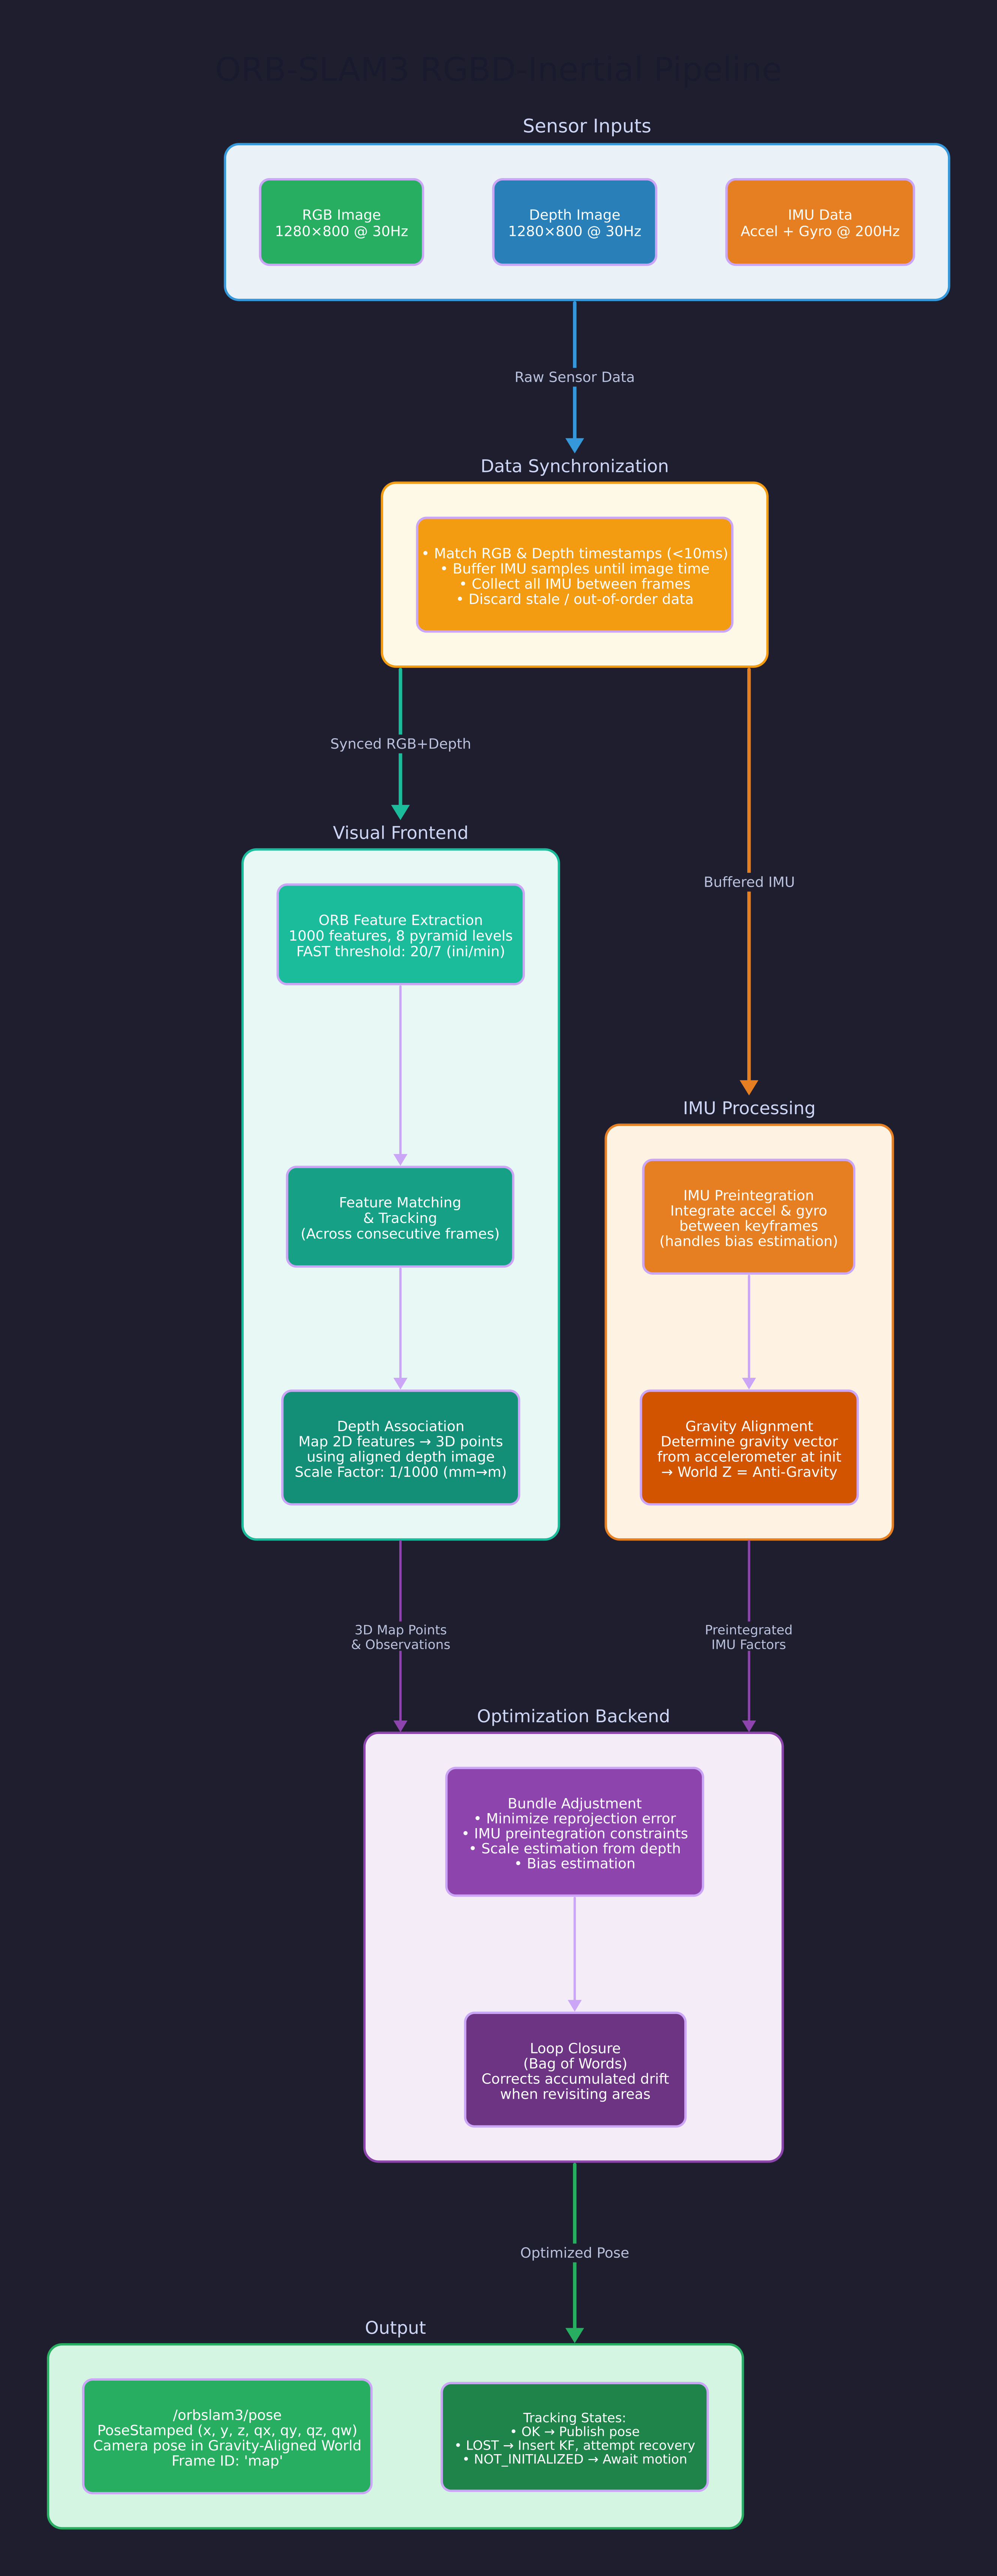
\includegraphics[width=\linewidth,height=0.75\textheight,keepaspectratio]{images/06_orbslam3_pipeline.jpg}
    \caption{ORB-SLAM3 RGBD-Inertial Processing Pipeline}
    \label{fig:data_flow}
\end{figure}

\subsubsection{Processing Pipeline}
\begin{enumerate}
    \item \textbf{Data Synchronization:} RGB and depth frames are matched within 10\,ms tolerance. IMU measurements are buffered and associated with the nearest image timestamp.
    \item \textbf{Feature Extraction:} ORB features are extracted from the RGB image --- 1000 features across 8 pyramid levels (scale factor 1.2), with adaptive FAST thresholds (initial: 20, minimum: 7).
    \item \textbf{Depth Association:} Each detected 2D feature is associated with its depth value from the aligned depth map, creating 3D landmarks with known metric scale.
    \item \textbf{IMU Preintegration:} Accelerometer and gyroscope measurements between consecutive frames are preintegrated to predict inter-frame motion, providing short-term odometry even when visual tracking is poor.
    \item \textbf{Tracking \& Optimization:} The system performs local Bundle Adjustment, jointly optimizing camera poses, 3D landmarks, and IMU biases to minimize reprojection error and inertial residuals.
    \item \textbf{Gravity Alignment:} During initialization, the IMU accelerometers determine the gravity vector. The world frame is rotated so its Z-axis aligns with vertical (against gravity), producing a horizon-level reference.
    \item \textbf{Loop Closure:} Bag-of-Words place recognition detects revisited locations and triggers a global pose-graph optimization to correct accumulated drift.
\end{enumerate}

\subsubsection{Key Configuration Parameters}
The ORB-SLAM3 configuration was optimized specifically for the Orbbec Gemini 2L camera's characteristics (file: \texttt{Orbbec\_Gemini2L\_Optimized.yaml}):

\begin{table}[H]
\centering
\scriptsize % reduces font size
\caption{ORB-SLAM3 Configuration Parameters}
\resizebox{\textwidth}{!}{%
\begin{tabular}{|p{4.2cm}|p{4.2cm}|p{7.4cm}|}
\hline \textbf{Parameter} & \textbf{Value} & \textbf{Justification} \\

\hline Camera1.fx / fy & 606.96 / 607.11 & Focal lengths from device intrinsic calibration \\

\hline Camera1.cx / cy & 637.73 / 392.85 & Principal point from device calibration \\

\hline Distortion ($k_1$--$k_3$, $p_1$--$p_2$) & -0.897, 0.252, 0.000, -0.001, 0.037 & Plumb-bob distortion model correcting barrel distortion \\

\hline RGBD.DepthMapFactor & 1000.0 & Converts depth from millimeters (sensor native) to meters \\

\hline Stereo.b (baseline) & 0.10 m & 100\,mm stereo baseline of the Gemini 2L \\

\hline IMU.NoiseGyro / NoiseAcc & 2.0e-2 / 2.0e-1 & Tuned higher than datasheet --- improves stability when stationary \\

\hline IMU.Frequency & 200 Hz & Matches camera IMU output rate \\

\hline IMU.fastInit & 0 (disabled) & Allows more robust initialization; avoids premature lock with noisy IMU \\

\hline \end{tabular}}
\label{tab:orbslam3_config_params}
\end{table}

\subsection{VIO Bridge - Frame Transformation \& Yaw Correction}
The VIO Bridge is a custom ROS 2 C++ node (\texttt{vio\_bridge\_node.cpp}) that serves as the critical middleware between the SLAM system and the flight controller. It performs three essential functions: coordinate frame rotation, heading alignment, and health monitoring.

\begin{figure}[!ht]
    \centering
    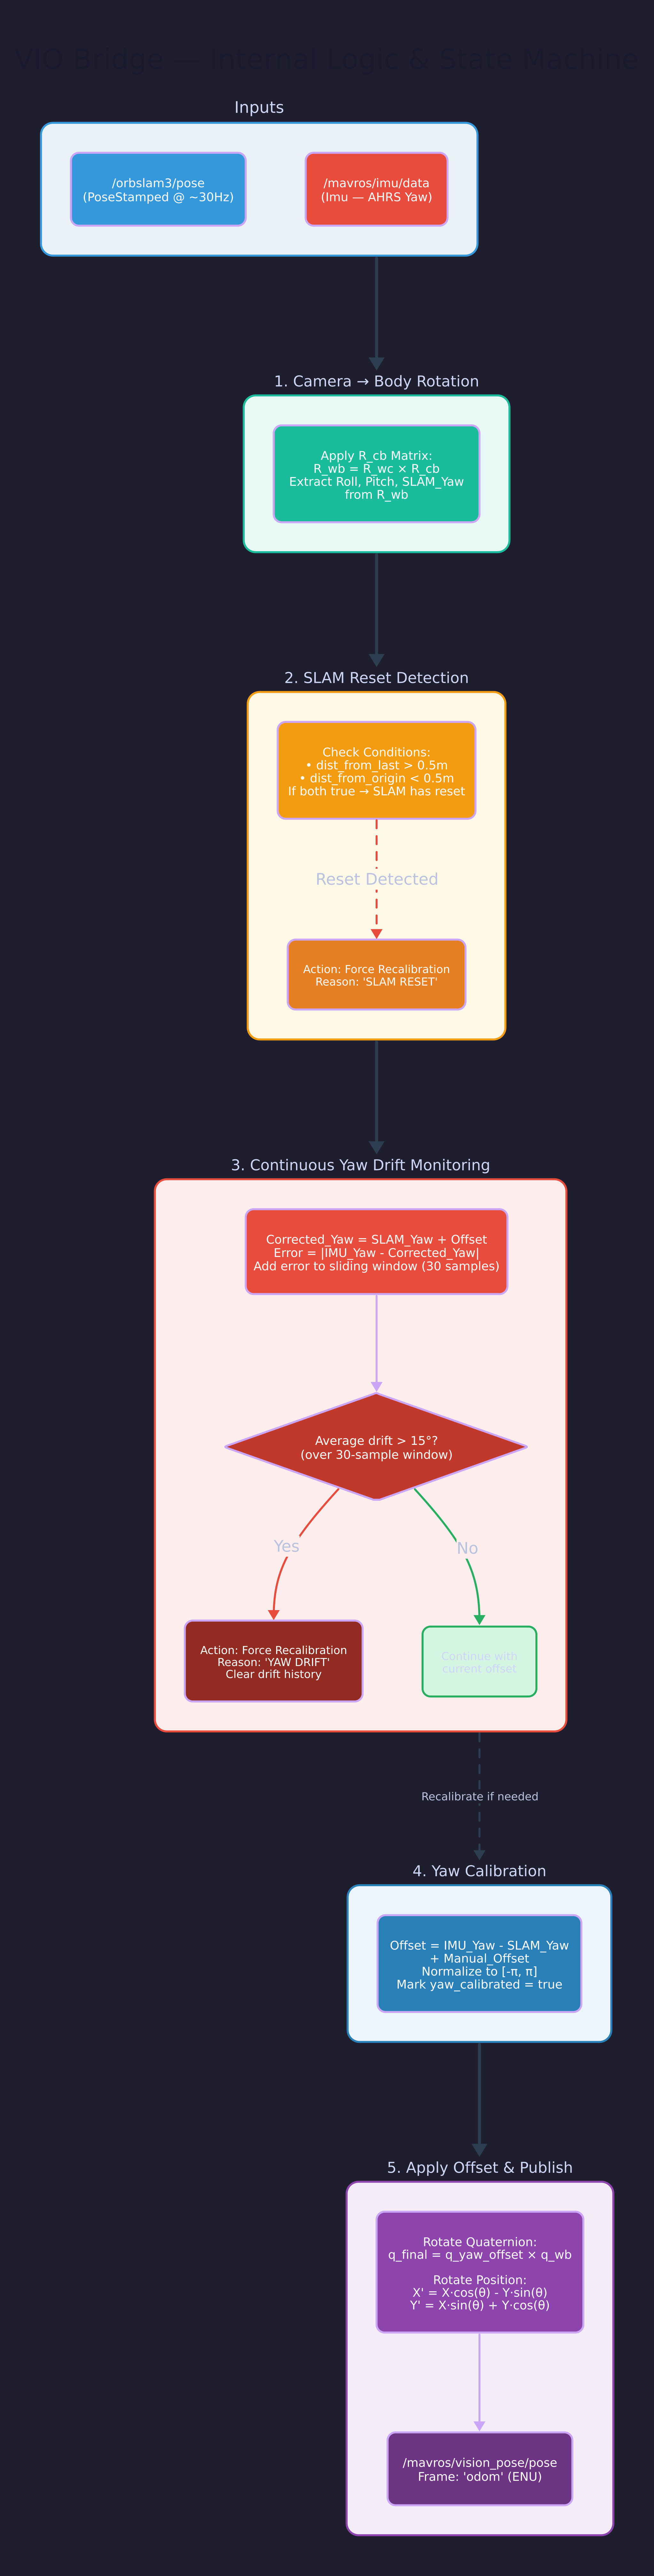
\includegraphics[width=\linewidth,height=0.75\textheight,keepaspectratio]{images/05_vio_bridge_logic.jpg}
    \caption{VIO Bridge Internal Logic }
    \label{fig:data_flow}
\end{figure}

\subsubsection{Camera-to-Body Frame Rotation}
\noindent ORB-SLAM3 outputs the camera pose in an Optical Frame convention (Right-Down-Forward, RDF). The flight controller expects poses in a Body Frame convention (Forward-Left-Up, FLU) aligned with the East-North-Up (ENU) world. The bridge applies a static rotation matrix $R_{cb}$:
\[
R_{cb} =
\begin{pmatrix}
0 & -1 & 0 \\
0 & 0 & -1 \\
1 & 0 & 0
\end{pmatrix}
\]
This maps:
\begin{itemize}
    \item Camera $Z$ (Forward) $\rightarrow$ Body $X$ (Forward)
    \item Camera $X$ (Right) $\rightarrow$ Body $-Y$ (Right, since Body $Y$ is Left)
    \item Camera $Y$ (Down) $\rightarrow$ Body $-Z$ (Down, since Body $Z$ is Up)
\end{itemize}
The full transformation is:
\[
T_{wb} = T_{wc} \times T_{cb},
\]
converting the World-to-Camera pose into a World-to-Body pose.

\subsubsection{Yaw Heading Correction}
ORB-SLAM3 initializes with an arbitrary yaw (Yaw = 0 at startup), which does not correspond to any real-world heading. PX4 requires that the vision pose heading is consistent with its internal heading estimate (derived from the magnetometer via the AHRS). The bridge implements the following yaw alignment algorithm:
\begin{enumerate}
    \item \textbf{Subscribe:} to \texttt{/mavros/imu/data} to obtain the current AHRS yaw from PX4.
    \item \textbf{Calculate Offset:} $\textit{yaw\_offset} = \textit{IMU\_Yaw} - \textit{SLAM\_Yaw}$ (at the first valid pose or after recalibration).
    \item \textbf{Apply Correction:} Rotate both the orientation quaternion and the position vector by the yaw offset. This ensures the entire trajectory is rotated to align with the real heading.
    \item \textbf{Position Rotation:} $x_{\text{final}} = x\cdot\cos(\textit{offset}) - y\cdot\sin(\textit{offset});\; y_{\text{final}} = x\cdot\sin(\textit{offset}) + y\cdot\cos(\textit{offset})$. This accounts for the fact that the SLAM coordinate axes must also be rotated, not just the heading.
\end{enumerate}

\subsubsection{Continuous Drift Monitoring}
SLAM heading can drift over time relative to the magnetometer. The bridge implements a sliding-window drift detector:
\begin{itemize}
    \item \textbf{Window Size:} 30 samples --- the bridge tracks the absolute yaw error between the corrected SLAM yaw and the IMU yaw over the last 30 SLAM poses.
    \item \textbf{Threshold:} $15^\circ$ --- if the average drift across the window exceeds 15 degrees, the bridge triggers an automatic recalibration (re-computes the yaw offset).
    \item \textbf{Hysteresis:} After recalibration, the drift history is cleared to prevent oscillating corrections.
\end{itemize}

\subsubsection{SLAM Reset Detection}
If ORB-SLAM3 loses tracking and re-initializes, the position jumps back to the origin. This would cause a dangerous discontinuity for PX4. The bridge detects this condition by monitoring the position: if the distance from the previous position exceeds 0.5\,m \textbf{and} the distance from the origin is less than 0.5\,m, a ``SLAM Reset'' is declared and the yaw offset is immediately recalibrated.

\subsubsection{Diagnostics}
The bridge runs a diagnostic timer every 5 seconds that logs: current publish rate (Hz), average yaw drift (degrees), SLAM reset count, and drift recalibration count. This provides real-time health monitoring during flight.
